\chapter{Methodologies}

The accurate segmentation of dendrites and dendritic spines remains a central challenge in computational neuroanatomy. While recent advances in deep learning have yielded promising automated solutions, these methods often lack the flexibility and interactive control required to address the variability in imaging modalities, experimental conditions, and morphological complexity encountered in real-world neuroscience research. In this chapter, we present a systematic exploration of multiple \gls{SAM}-based architectures beginning with the original \gls{SAM} model, extending to parameter-efficient fine-tuning via \gls{LoRA}, and advancing to the temporally consistent \gls{SAMv2} before introducing our own Neuro-\gls{SAM} framework. Unlike prior fully automated approaches, Neuro-\gls{SAM} is an interactive, modular pipeline that unifies dendrite path tracing, dendrite segmentation, spine detection, and spine segmentation, enabling researchers to move seamlessly from raw volumetric imaging data to high-fidelity morphological reconstructions. Through this progression, we investigate how each methodological step contributes to accuracy, generalization, and annotation efficiency, culminating in a framework designed to answer our central research question.

\section{Data and Preprocessing}
The datasets used in this work were derived from the \gls{DeepD3} dataset \cite{Fernholz_2024}, an in-house curated collection of expert-annotated 3D microscopy image stacks capturing dendritic shafts and dendritic spines under varied imaging conditions. Each stack was manually annotated by three independent experts at single-pixel precision to mitigate annotator bias and promote generalization. Annotations encompassed both dendrites and dendritic spines, providing paired binary masks suitable for supervised segmentation. 

The datasets were designed to address one of the central challenges in neuronal morphology analysis: the extreme variability in imaging modalities, acquisition parameters, and biological structures. By incorporating data from multiple sources and experimental paradigms, this dataset enables the development of segmentation models that generalize beyond a single laboratory or imaging setup. The Table \ref{fig:dataset_description} shows the heterogeneity of imaging conditions for the training, validation and the benchmark dataset. This diversity was intentionally curated to force models to handle variations in spatial resolution, signal-to-noise ratio, and labeling characteristics.

\begin{center}
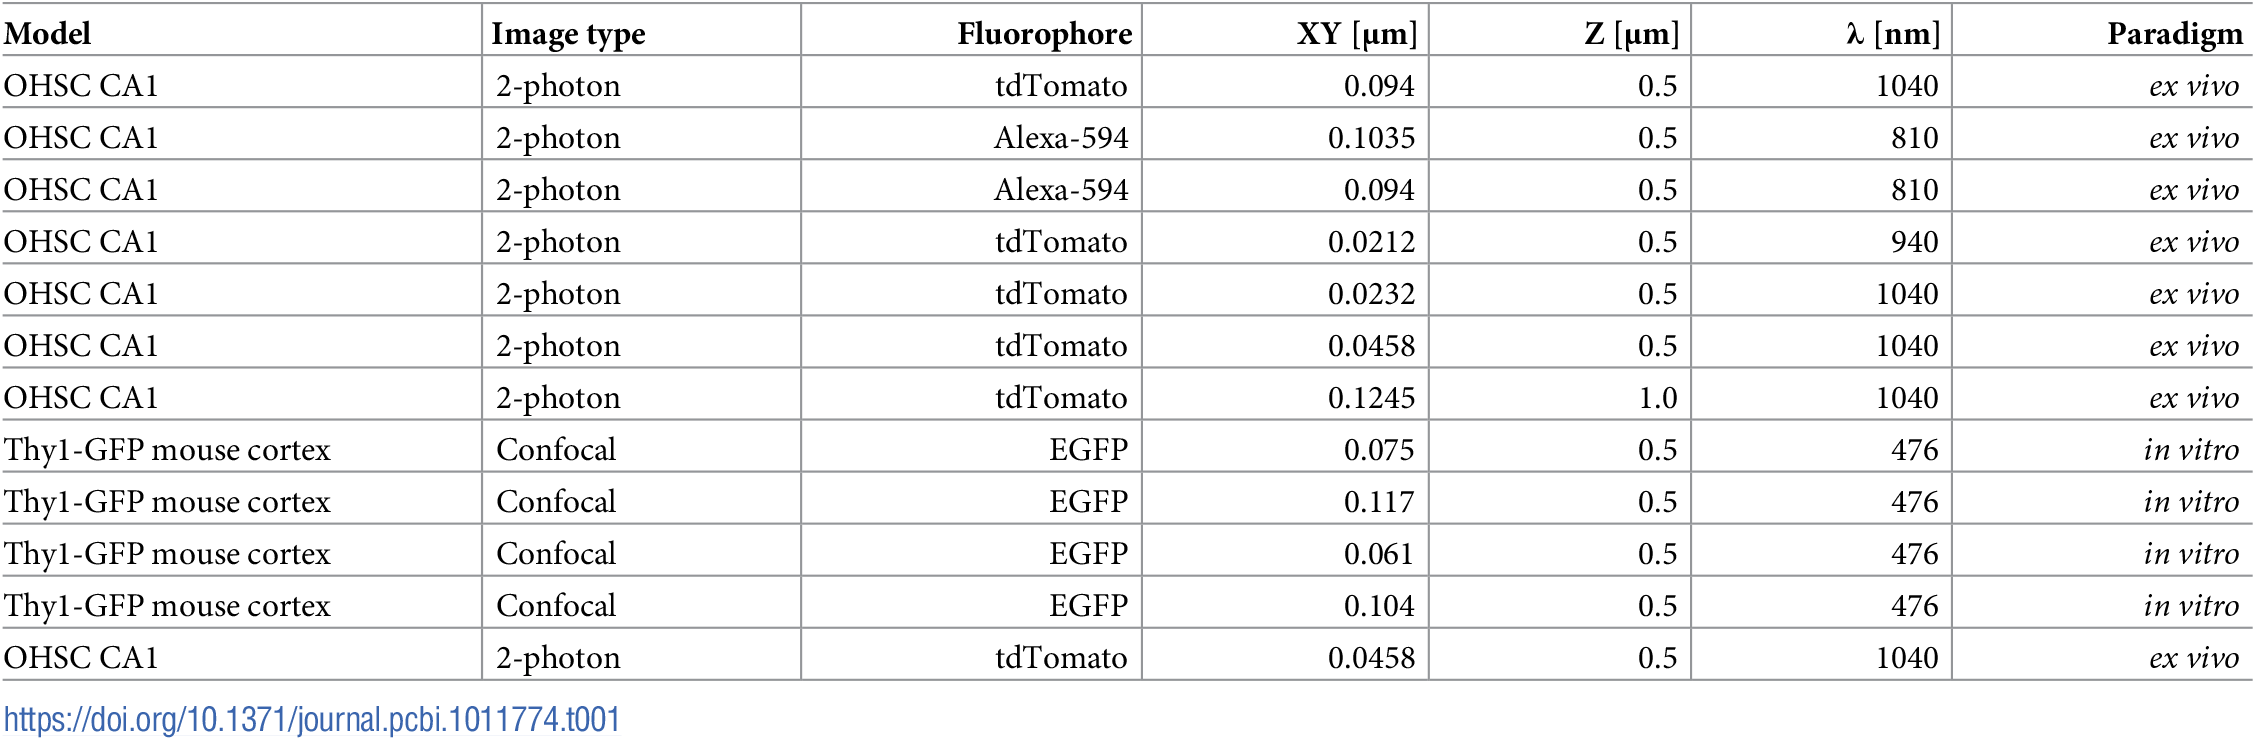
\includegraphics[width=0.95\textwidth]{figures/56_dataset_description.png}
\captionof{figure}{Overview of data (acquired from \cite{Fernholz_2024}), including model organism, brain region, microscopy type, resolution, and imaging wavelength ($\lambda$). Image source: \cite{Fernholz_2024}}
\label{fig:dataset_description}
\end{center}

% \subsubsection{\textbf{Heterogeneity of imaging conditions}}
% The dataset contains 3D image stacks from:
% \begin{itemize}
% \item \textbf{Microscopy types:} confocal, ex vivo two-photon, and in vivo two-photon imaging.
% \item \textbf{Species:} both mouse and rat preparations.
% \item \textbf{Brain regions:} hippocampal CA1 and mouse cortex.
% \item \textbf{Fluorophores:} tdTomato, Alexa-594, EGFP.
% \item \textbf{Voxel sizes (XY):} from 0.0212~$\mu$m to 0.1245~$\mu$m; \textbf{Z-step sizes:} 0.5–1.0~$\mu$m.
% \item \textbf{Excitation wavelengths:} 476–1040~nm.
% \item \textbf{Cell type:} exclusively pyramidal neurons.
% \end{itemize}


\subsubsection{\textbf{Data Annotations}}
To ensure the highest possible annotation fidelity, three expert raters reconstructed the dendritic shafts in three dimensions using NeuTube \cite{Feng_2015}, generating SWC format \cite{Cannon_1998} skeletons that encoded both topology and diameter. The SWC format represents neuronal morphology as a directed tree model, where each node specifies spatial coordinates, radius, and connectivity. A custom Python toolbox interpolated spheres along these traces to produce volumetric dendrite masks aligned with the image data. Dendritic spines, often approaching the resolution limits of light microscopy, were manually segmented using \gls{PiPrA} \cite{Anki_Pipra}, producing precise binary masks. This dual-annotation process ensured that both coarse and fine structural elements were captured.

\subsubsection{\textbf{Training and validation split}}
The dataset was divided into training and validation subsets at the stack level, guaranteeing that no image stack appeared in both sets. The training subset spanned the full range of modalities, species, and resolutions. During training, stacks were dynamically tiled into 128$\times$128~px patches, each paired with binary masks for dendrites and spines. The validation subset preserved the heterogeneity of the training data while remaining completely independent, providing an unbiased measure of model generalization.

Because the \gls{DeepD3} dataset encompasses multi-modal, multi-species, and multi-resolution data, it served as a robust foundation for all experiments in this chapter. Every model \gls{SAM}, \gls{SAM}+\gls{LoRA}, \gls{SAMv2}, and Neuro-\gls{SAM} was trained and validated exclusively on this dataset, enabling fair comparison across architectures and ensuring that observed performance differences arise from methodological changes rather than data variability.

\subsection{Benchmark Dataset}
The \gls{DeepD3} benchmark dataset \cite{Fernholz_2024} was used as the exclusive evaluation set, fully independent of the training and validation data. It was deliberately designed to capture diverse imaging conditions, species, and anatomical regions, providing a stringent test of model generalization. All annotations were produced by multiple experts, with consensus labeling applied to minimize variability and ensure reliability. This combination of heterogeneity and expert fidelity made the benchmark the most rigorous evaluation standard in this study, and all quantitative results are reported on this dataset.

\subsection{Preprocessing}
All microscopy stacks followed a consistent preprocessing pipeline before training. Image stacks were resampled, when necessary, to match the target spatial resolution specified in the metadata, ensuring uniformity across modalities and acquisition systems. Cropping and tiling were performed dynamically during training, where $128 \times 128$~px patches were extracted from random locations within each stack. This online streaming strategy provided a continuous supply of varied samples without requiring large preprocessed datasets to be stored on disk. Each patch was normalized to a fixed intensity range to reduce variability in brightness and contrast across imaging sessions. For stacks acquired at different voxel resolutions, spatial dimensions were proportionally scaled to preserve the physical dimensions of neuronal structures in microns. Binary masks for dendrites and spines were generated from volumetric annotations and resized using the same interpolation settings as the corresponding images, maintaining pixel-perfect alignment.

\subsection{Data Augmentation}
To enhance robustness and mitigate overfitting, data augmentations were applied on-the-fly during training. Geometric transformations included small-angle rotations, random $90^\circ$ rotations, and horizontal or vertical flips. Photometric augmentations consisted of brightness and contrast adjustments, Gaussian blur, and Gaussian noise addition. All augmentations were applied consistently to both the microscopy images and their corresponding binary masks, preserving annotation fidelity. This strategy ensured that training and validation data shared a uniform format while maintaining variability, enabling fair and reliable performance comparisons across model architectures.

The same preprocessing pipeline and augmentation strategy were applied to all models fine-tuned in this thesis. This ensured that differences in performance reflect methodological variations between models rather than inconsistencies in data preparation.

\section{Model Architectures and Experimental Setup}
Building on the datasets and preprocessing described earlier, we now investigate how different foundation models configurations perform in dendritic structure segmentation. Beyond accuracy, the aim is to understand how architectural choices and fine-tuning strategies affect a model’s ability to capture thin dendrites and small, low-contrast spines. Our experiments progress from the \gls{SAM} model to parameter-efficient fine-tuning with \gls{LoRA}, then to the temporally consistent \gls{SAMv2}, before introducing Neuro-\gls{SAM}, our interactive, modular pipeline for dendrite and spine analysis.

All models were trained and validated on the same heterogeneous dataset and tested on the benchmark set, ensuring fair, direct comparison. We begin with \gls{SAM} in its original form, exploring both zero-shot and fine-tuned performance as a baseline for the more specialized approaches that follow.

\subsection{Segment Anything Model}
Our first set of experiments with \gls{SAM} focused on evaluating its ability to segment dendrites in both a zero-shot setting and after fine-tuning on our dataset. The goal was to establish a clear performance baseline of the foundation models and to measure the gains achievable through domain-specific adaptation.

\subsubsection{\textbf{Zero-shot Evaluation}}
In the zero-shot stage, \gls{SAM} was applied directly to the \gls{DeepD3} benchmark dataset using an automated grid-based prompting strategy. Positive prompts were placed at evenly spaced intervals across the field of view, ensuring uniform coverage of the image. This method provided an unbiased probe into \gls{SAM}’s pretrained capabilities without any influence from our dataset. The resulting segmentations highlighted both the strengths and limitations of the model when confronted with fine-scale neuronal morphology for which it was not explicitly trained.

\subsubsection{\textbf{Fine-tuning}}
For fine-tuning, we implemented a custom PyTorch dataloader tailored to our training data format. Multi-page \gls{TIFF} files containing paired grayscale images and binary dendrite masks were streamed dynamically during training, avoiding the need to pre-tile and store patches on disk. Each image slice was normalized to the range $[0,1]$ and resized when necessary to match the target resolution. Ground truth masks were processed in parallel to generate training prompts. We trained the model for 80 epochs with a batch size of 8 and the learning rate was set to $2 \times 10^{-5}$. The training and validation curves are provided in Appendix \ref{sec:sam_plots} for reference.

\subsubsection{\textbf{Prompt Generation}}
Prompt generation was handled by sampling \textit{positive} points from connected components in the dendrite masks and \textit{negative} points were obtained from surrounding background regions through morphological dilation. This ensured that the model was exposed to both inclusion and exclusion cues in every training iteration. When no valid points could be identified, default coordinates were provided to maintain training stability.

% \subsubsection{\textbf{Data Augmentation}}
% On-the-fly data augmentation was performed using the Albumentations library, including small-angle rotations, random 90° rotations, horizontal and vertical flips, brightness and contrast adjustments, Gaussian blur, and Gaussian noise injection. Augmentations were applied consistently to both images and masks to preserve spatial alignment between inputs and labels. This augmentation strategy was essential for improving model robustness to the diverse imaging conditions present in our dataset.

% \subsubsection{\textbf{Evaluation}}
% The fine-tuned \gls{SAM} was trained on the training set, validated on its dedicated validation split, and finally evaluated on the benchmark dataset. The evaluation used the same grid-based prompting strategy as the zero-shot experiment to ensure direct comparability. No post-processing was applied to the outputs, meaning that the reported results reflect the model’s raw segmentation performance.

\subsection{Segment Anything Model + Low Rank Adaptation}
To further adapt \gls{SAM} to the morphological and contrast characteristics of dendritic imaging while maintaining a manageable training footprint, we integrated \gls{LoRA} layers into the \gls{SAM} image encoder. This approach allowed selective fine-tuning of a small set of parameters, preserving the majority of the pretrained weights while steering the model towards domain-specific features present in the dataset. All experiments were implemented within our custom training framework, which was developed to streamline model configuration, dataset handling, and evaluation across different \gls{SAM} variants.

\subsubsection{\textbf{Architecture}}
This approach builds upon the original \gls{SAM} framework by selectively fine-tuning the image encoder through \gls{LoRA}, while keeping the prompt encoder and mask decoder completely frozen. The model architecture (\autoref{fig:sam_lora_arch}) originally designed for retinal capillaries was fine-tuned for our purpose \cite{Wang_2023}. The model receives an input microscopy slice along with automatically extracted prompt points in the form of 2D coordinates. Positive and negative prompts are encoded into a learned spatial representation using a Gaussian positional encoding scheme and passed through the frozen prompt encoder.

The input image is processed by a \gls{ViT}-based image encoder where \gls{LoRA} modules are injected into each self-attention block. These modules introduce a pair of trainable low-rank matrices within the \gls{MLP} projections, allowing efficient adaptation of the encoder without modifying the pretrained backbone weights. Only these \gls{LoRA} parameters are updated during training, significantly reducing the total trainable parameter count while maintaining the benefits of the original \gls{SAM} pretraining.

The image and prompt features are merged and forwarded to the frozen mask decoder, which consists of a transformer followed by two prediction heads: one for estimating mask quality and one for generating the binary segmentation mask. The prediction is compared to the ground truth dendrite mask using a segmentation loss, without any need for decoder fine-tuning. This modular setup allows isolated adaptation of the image encoder to domain-specific signals while preserving the integrity of the rest of the foundation model.

\begin{center}
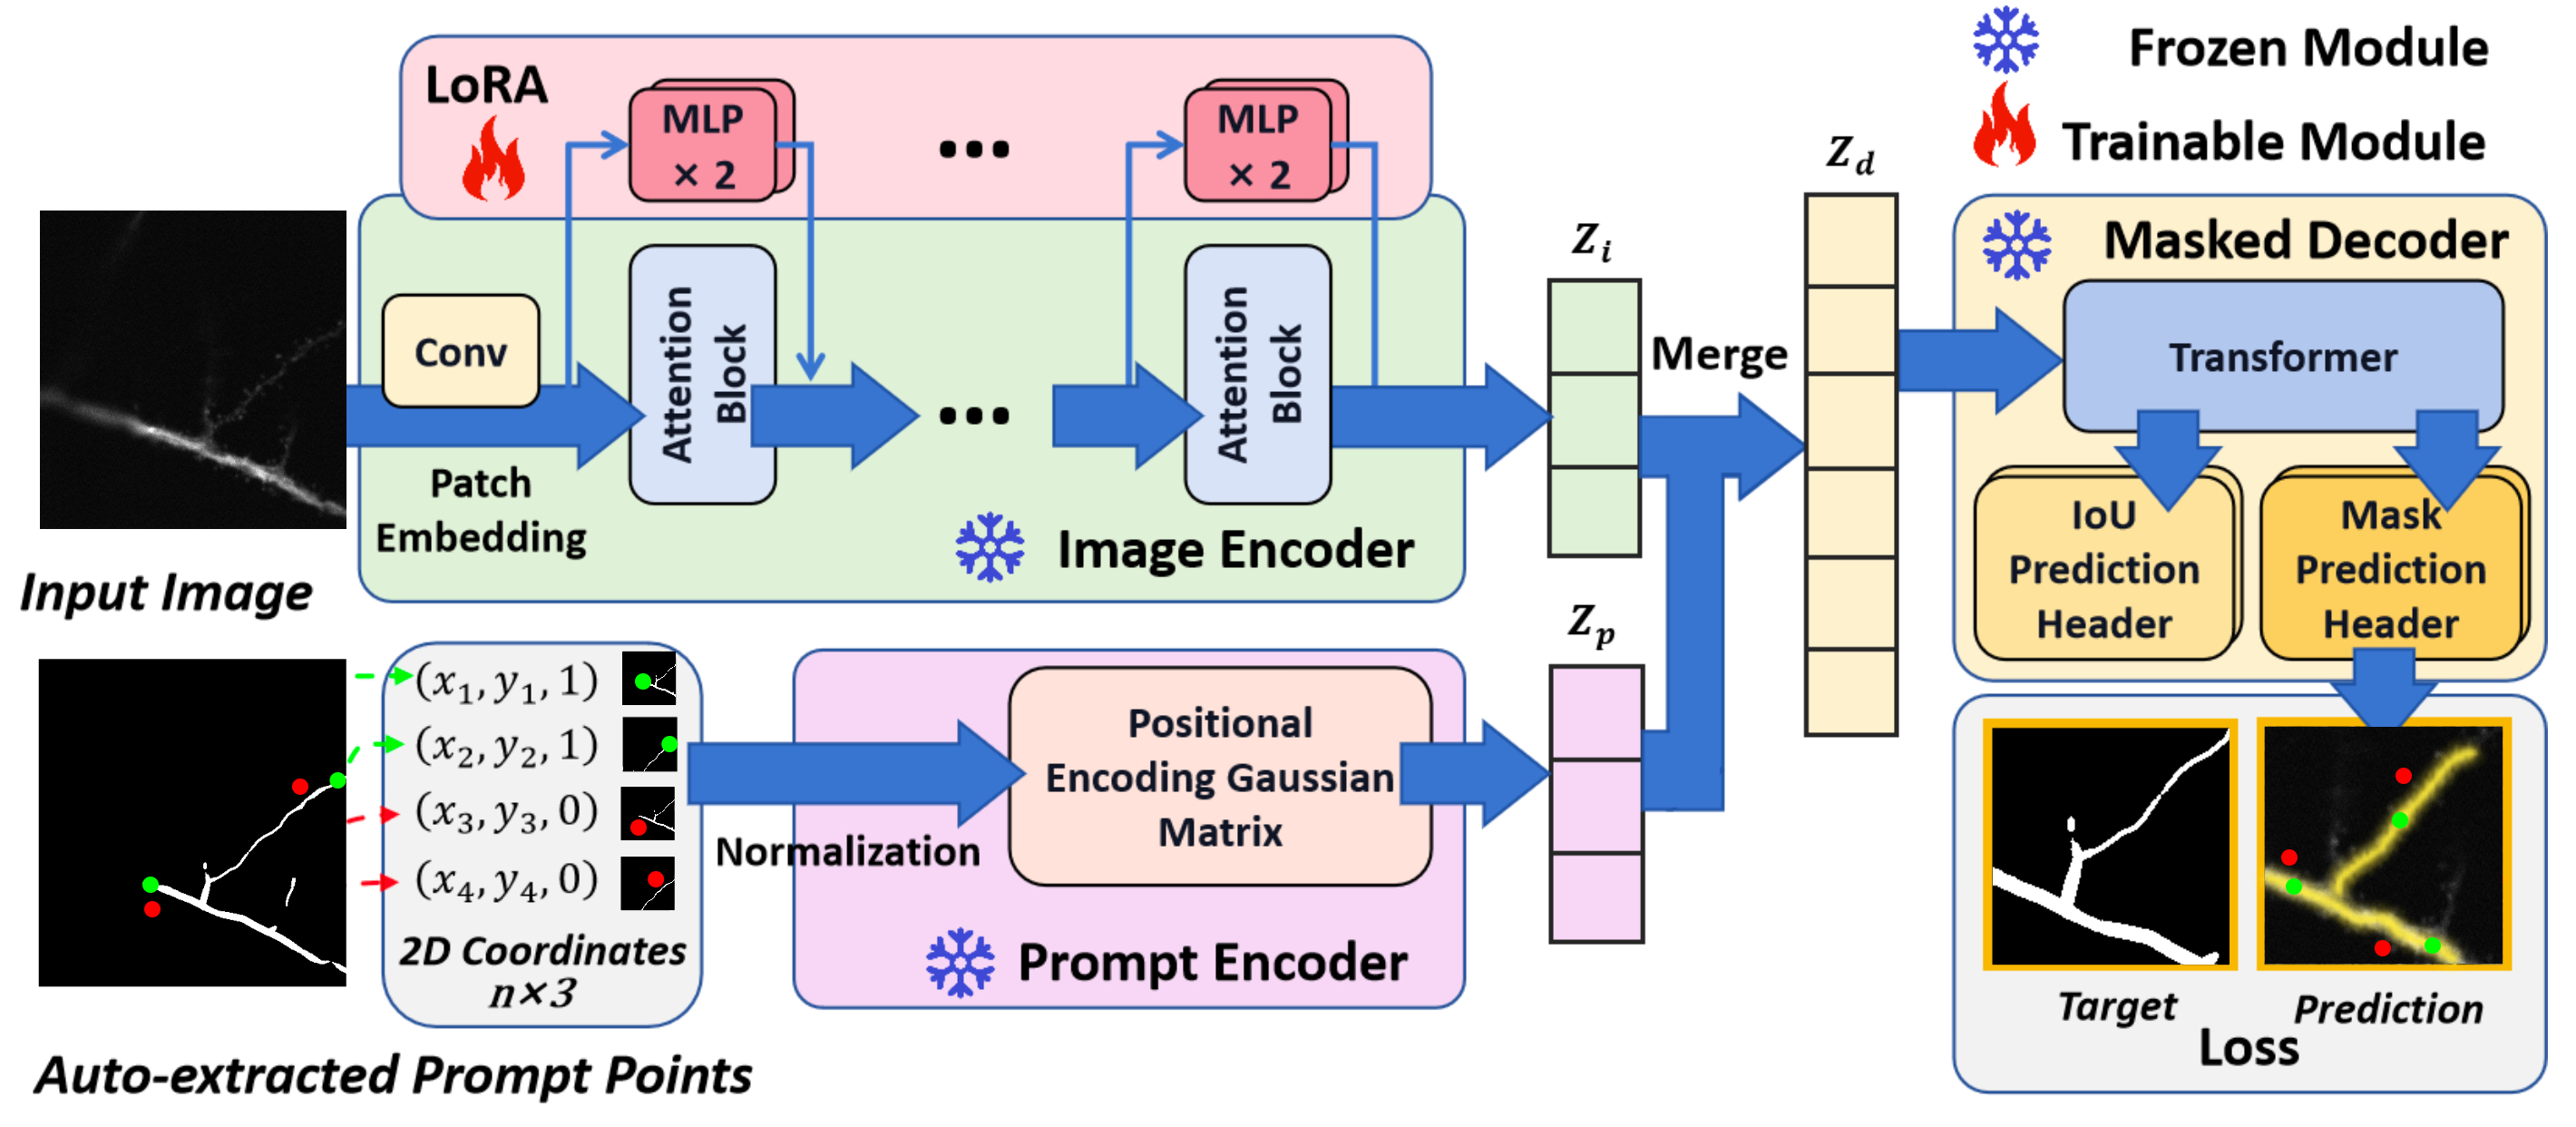
\includegraphics[width=0.95\textwidth]{figures/14_sam_lora_arch.jpg}
\captionof{figure}{Training architecture for \gls{SAM}+\gls{LoRA}. Only the \gls{LoRA} adapters in the image encoder are trainable (marked in red); the prompt encoder and decoder remain frozen. Automatically extracted positive (green) and negative (red) points are encoded and fused with image features to predict the dendrite mask. Image adapted from: \cite{Wang_2023}}
\label{fig:sam_lora_arch}
\end{center}

\subsubsection{\textbf{Fine-tuning Setup}}
For \gls{SAM}+\gls{LoRA}, fine-tuning was implemented by injecting \gls{LoRA} modules into the attention blocks of \gls{SAM}’s image encoder. Each attention block was modified by adding two trainable low-rank matrices ($A \in \mathbb{R}^{d \times r}$ and $B \in \mathbb{R}^{r \times d}$, where $r = 4$ and $d$ is the hidden dimension of the projection), which were inserted into the \gls{MLP} projections. This allowed us to adapt the model to the dendritic segmentation task while keeping the majority of \gls{SAM}’s parameters frozen. The prompt encoder and mask decoder were entirely fixed during training, ensuring that the core behavior of \gls{SAM} remained stable. The only learnable weights were the \gls{LoRA} parameters, resulting in a lightweight training setup with approximately 0.2\% of the full model being updated.

The entire training pipeline was implemented in PyTorch within a custom framework developed. The entry points for training and evaluation were handled through training and testing scripts, while model configuration including \gls{LoRA} rank, learning rate, \gls{GPU} usage, logging behavior, and checkpoint naming was controlled through a config file. This modularity allowed rapid experimentation across different architectural variants. The training was performed on a NVIDIA A100 \gls{GPU} (40 GB memory), using mixed-precision (FP16) acceleration for efficiency.

Training was carried out over 50 epochs with a batch size of 8. The optimizer used was AdamW with a learning rate of $2 \times 10^{-5}$ and weight decay of $10^{-4}$. A cosine annealing scheduler was used to gradually decrease the learning rate over the course of training. Checkpoints were saved every 5 epochs for evaluation. Logs and metrics were stored both locally and optionally through Weights \& Biases for experiment tracking.

Input data consisted of 2D image slices and their corresponding binary dendrite masks, streamed from multi-page \gls{TIFF} stacks. A custom PyTorch \texttt{DatasetLoader} class handled data streaming and augmentation. Each slice was normalized to the range $[0,1]$ using min–max scaling and resized to $1024 \times 1024$ to match the expected model input size. For each image-mask pair, prompt points generated online (positive/negative) were passed to the frozen prompt encoder, and the resulting embeddings were merged with the image features in the transformer encoder–decoder pipeline.

The output segmentation mask was supervised using a composite loss function consisting of binary cross-entropy and soft Dice loss, equally weighted \cite{Galdran_2022}. This combination helped balance pixel-level precision and region-level overlap. Importantly, only the \gls{LoRA} parameters received gradient updates, neither the backbone, nor the prompt encoder, nor the decoder were modified. This ensured that all architectural and performance improvements came strictly from \gls{LoRA} adaptation.

This strict isolation of \gls{LoRA}-based fine-tuning, combined with consistent preprocessing, prompting, and loss across experiments, allows direct comparisons to both the original \gls{SAM} and later variants. The final trained models were stored under structured experiment directories and evaluated using the same benchmark protocol as all other models in this work.

% \subsubsection{\textbf{Data Augmentation}}
% To improve robustness and prevent overfitting, a set of on-the-fly augmentations was applied to each input image–mask pair during training. Augmentations were implemented using the Albumentations library and included both geometric and photometric transformations. Geometric operations involved small-angle random rotations (up to $\pm10^\circ$), random 90° rotations, and horizontal and vertical flips. These transformations simulated the natural orientation variance found in microscopy stacks. Photometric augmentations included brightness/contrast adjustments, Gaussian blur, and additive Gaussian noise, helping the model remain resilient to changes in illumination conditions and imaging noise commonly observed across different acquisition sessions.

% All augmentations were applied synchronously to both the grayscale input image and the corresponding dendrite mask, preserving pixel-wise alignment throughout the pipeline. Since prompt points were extracted from the binary mask, it was critical that augmentations were applied \textit{before} prompt generation to ensure spatial consistency. The augmentation operations were applied stochastically for each training patch, resulting in a diverse and unpredictable sampling of augmented views across training epochs. This augmentation policy was kept consistent across all experiments to ensure that any performance differences could be attributed to the model architecture or training strategy rather than changes in input distribution.

\subsubsection{\textbf{Prompt Generation}}
During training, prompt points were generated on-the-fly from the ground truth dendrite masks. For each connected component in the binary mask, one or more positive points were randomly sampled from within the foreground region. Negative prompts were selected from a morphologically dilated boundary surrounding the structure. This contrastive prompting ensured the model received both inclusion and exclusion signals, helping it learn spatial boundaries even in noisy or low-contrast microscopy contexts. All prompts were encoded as $(x, y)$ coordinates with associated binary labels, and passed to the frozen \gls{SAM} prompt encoder.

At test time, prompts were generated directly from the input image using OpenCV’s \texttt{goodFeaturesToTrack} corner detection algorithm \cite{Shi_1994}. The \autoref{fig:sam_lora_prompt_points} shows that a fixed number of \textit{positive points} were extracted from regions of high spatial contrast, ensuring coverage of salient features. To provide negative supervision, the algorithm also sampled an equal number of low-intensity pixels below the mean of the image, treating them as background cues. This method required no access to ground truth annotations during inference and allowed fully automated segmentation at test time. The prompt points were encoded, fused with image features, and forwarded through the frozen decoder to produce segmentation masks. 

\begin{center}
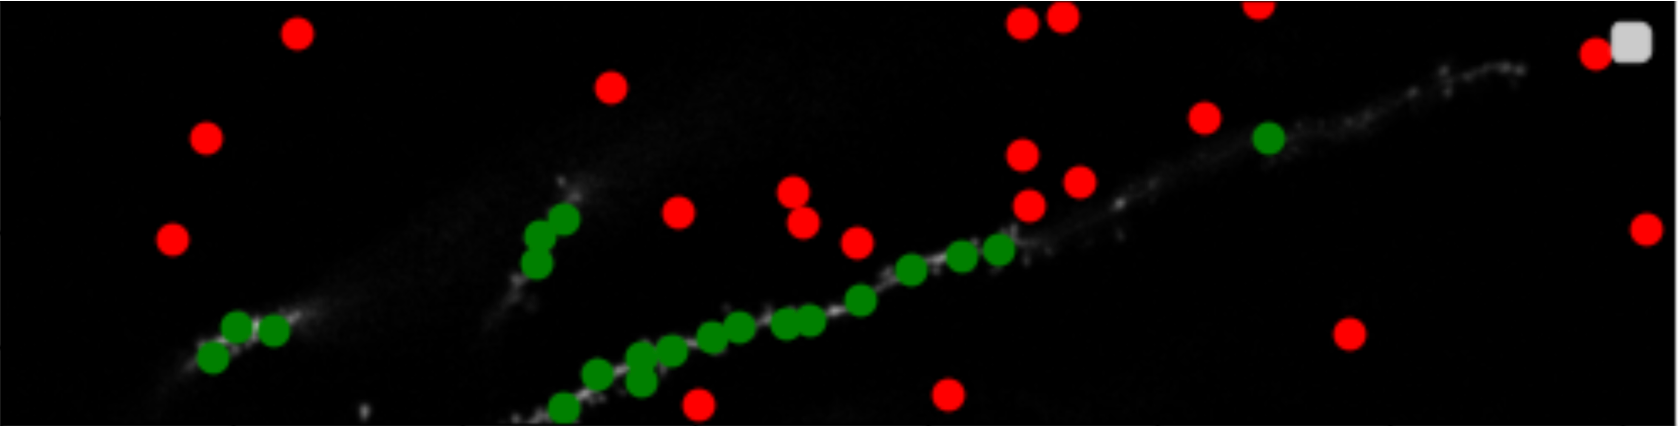
\includegraphics[width=0.95\textwidth]{figures/57_bimap_prompt_points.png}
\captionof{figure}{Prompt Points for \gls{SAM}+\gls{LoRA}. Automatically extracted positive (green) and negative (red) points serves as the prompts for our model. Scale: $0.94\,\mu\text{m}/\text{px}$}
\label{fig:sam_lora_prompt_points}
\end{center}

% \subsubsection{\textbf{Evaluation}}
% \gls{SAM}+\gls{LoRA} was evaluated on the benchmark dataset, entirely separate from the training and validation sets. Each 2D slice was normalized and passed through the model along with prompt points automatically generated from the input image. Positive prompts were extracted using OpenCV’s \texttt{goodFeaturesToTrack} method \cite{Shi_1994}, which identified corners in regions of high local contrast. Negative prompts were sampled randomly from low-intensity background pixels. The model’s outputs were thresholded at 0.5 and saved as binary masks. When ground truth was available, Dice and IoU scores were computed per slice and averaged across the stack. The entire evaluation pipeline was fully automated and logged under timestamped directories for reproducibility

\subsection{Segment Anything Model 2}
All interactive segmentation within the Neuro-\gls{SAM} framework was built upon Segment Anything Model 2, a recent extension of the original \gls{SAM} that introduces temporal and spatial consistency through a memory attention mechanism. While earlier experiments in this work explored standard \gls{SAM} and its low-rank adaptation (\gls{LoRA}) for dendrite segmentation, \gls{SAMv2} was chosen as the backbone model for the final interactive pipeline due to its ability to operate across volumetric data and maintain consistency across slices. Unlike \gls{SAM} and \gls{SAM}+\gls{LoRA}, \gls{SAMv2} was not benchmarked in isolation; instead, it was directly fine-tuned and integrated into our dendrite and spine segmentation modules, which together constitute the core of Neuro-\gls{SAM}.

\subsubsection{\textbf{Architecture}}
While the original \gls{SAM} and its \gls{LoRA}-based adaptation provided strong capabilities, they lacked a mechanism for handling volumetric continuity, something critical for dendritic analysis in 3D microscopy stacks. \gls{SAMv2} addresses this limitation by introducing a memory attention mechanism that allows the model to incorporate contextual information from neighboring slices. This is particularly useful when segmenting dendritic shafts that may span multiple frames but appear intermittently due to signal dropout or imaging noise. In Neuro-\gls{SAM}, this architecture proved instrumental in preserving topological consistency and reducing frame-wise segmentation drift. By integrating both short-range and long-range dependencies across z-slices, \gls{SAMv2} served as the structural backbone for the entire interactive pipeline, supporting both dendrite and spine segmentation in 3D.

\subsubsection{\textbf{Role in Neuro-\gls{SAM}}}
\gls{SAMv2} served as the core segmentation model within the Neuro-\gls{SAM} pipeline. Two instances of the \gls{SAMv2} architecture were separately fine-tuned: one for dendrite segmentation and another for spine segmentation. This modular reuse allowed the model to be tailored to the structural and visual characteristics of each task while maintaining architectural consistency across the pipeline. Both fine-tuned variants leveraged \gls{SAMv2}’s memory-based architecture to improve continuity across volumetric stacks. All training details, data handling procedures, prompt strategies, and post-processing steps involving \gls{SAMv2} are discussed in detail in the Neuro-\gls{SAM} section that follows.

\section{Neuro-SAM}
Building on the insights from previous experiments, Neuro-\gls{SAM} was developed as an interactive segmentation framework tailored specifically for dendritic structures and dendritic spines in volumetric microscopy data. Unlike static segmentation pipelines, Neuro-\gls{SAM} enables users to interactively trace individual dendrites, perform high-fidelity segmentation, detect spines in 3D, and segment them all within a unified interface. The framework is modular by design and leverages two independently fine-tuned instances of \gls{SAMv2}: one specialized for dendrite segmentation and the other for spine segmentation. Combined with a memory-aware architecture, automated prompt generation strategies, and a 3D visualization environment in Napari, Neuro-\gls{SAM} provides precise and adaptable segmentation capabilities that reflect the workflow of real neuroscience annotation tasks.

\subsection{System Overview}
Neuro-\gls{SAM} is designed as a modular, interactive framework for segmenting dendrites and dendritic spines from volumetric microscopy stacks. The system follows a linear yet flexible workflow that mirrors expert annotation practices: beginning with path selection, followed by dendrite segmentation, spine detection, and finally spine segmentation. Each of these steps is organized as a dedicated module within the Napari interface, allowing users to operate on individual dendritic paths with full visual and structural control.

\autoref{fig:neuro_sam} shows the pipeline with a raw 3D stack, where the user interactively traces one or more dendritic paths using an optimized A* algorithm guided by manually placed waypoints. These traced paths are then passed to a fine-tuned \gls{SAMv2} model for targeted dendrite segmentation. After post-processing, the system generates a localized tubular representation along the segmented dendrite to detect spines along its surface. Detected spines, along with any manually added corrections, are used as prompt points for a second fine-tuned \gls{SAMv2} model specialized for spine segmentation. At each step, users can visualize results in both 2D and 3D, iterate on inputs, and export masks for downstream use. The modular nature of the system allows for precise control over each stage of the segmentation process, aligning the model’s output with biological expectations.

\begin{center}
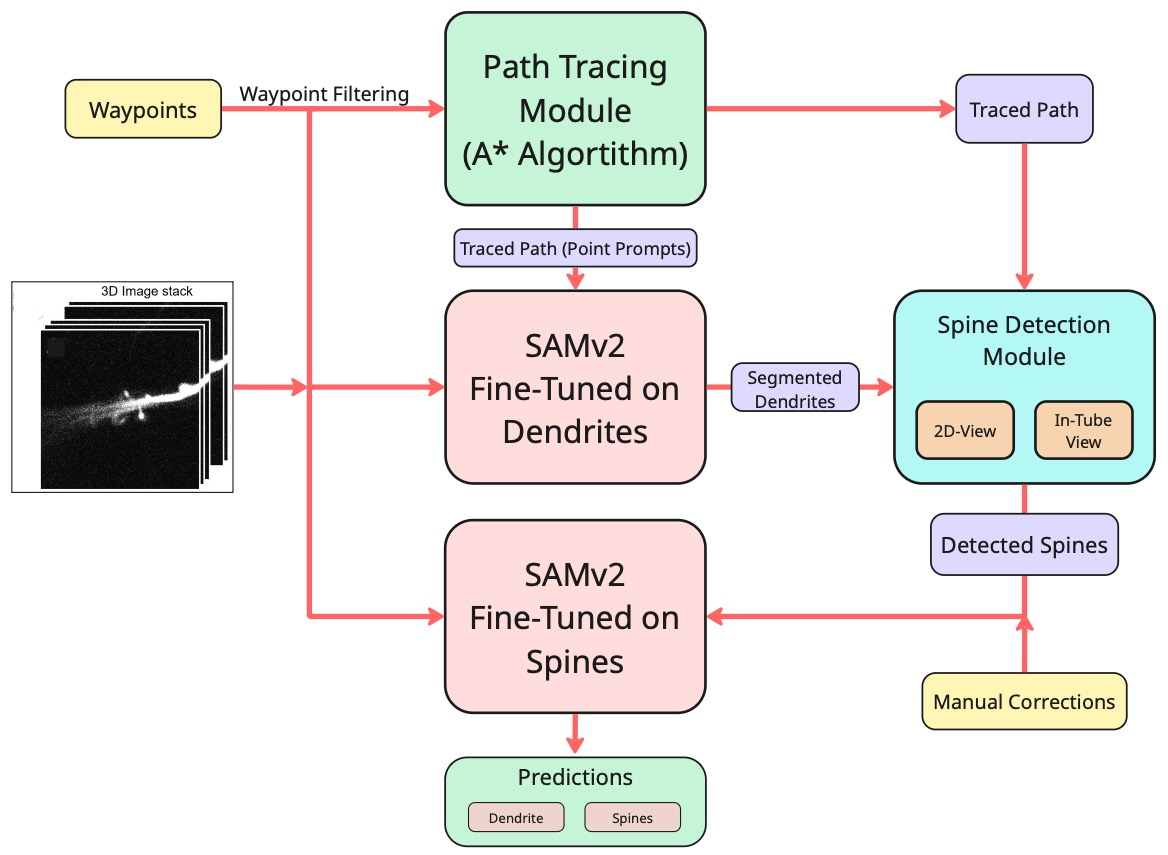
\includegraphics[width=0.95\textwidth]{figures/15_neuro_sam.jpg}
\captionof{figure}{Neuro-\gls{SAM} Pipeline. It takes the 3D stack and the waypoints as an input and produces segmentation masks for dendrites and dendritic spine.}
\label{fig:neuro_sam}
\end{center}

\subsection{Interactive Visualization and User Control}
The user interface of Neuro-\gls{SAM} is implemented entirely within the Napari framework, enabling real-time 2D and 3D visualization of volumetric image stacks alongside interactive annotation and segmentation modules. Upon launching the tool, users are presented with a configurable 3D viewer where raw microscopy stacks can be loaded and visualized as orthogonal slices. To accommodate heterogeneous voxel resolutions across datasets, the interface includes controls for adjusting \textit{X, Y,} and \textit{Z} scaling, ensuring that anisotropic stacks can be rendered and navigated proportionally. These rescaling operations affect both display and downstream processing, and are essential for maintaining spatial accuracy in path tracing and segmentation.

The modular nature of the framework is realized through a multi-tab panel on the right-hand side of the Napari interface. Each tab corresponds to a specific stage in the segmentation workflow including path tracing, dendrite segmentation, spine detection, and spine segmentation. This design enables users to work incrementally, focusing on one dendritic structure at a time without overloading the interface. Within each module, user actions are performed via buttons and mouse-based selections directly on the stack view. The state of the interface including traced paths, intermediate segmentations, and spine prompts is preserved across tabs, allowing users to iteratively refine results without losing context.

Crucially, Neuro-\gls{SAM} is designed around the principle of “guided interactivity”: the system does not require full-volume annotation or batch processing. Instead, it empowers the user to selectively trace and segment individual dendritic branches. This targeted approach reflects real-world annotation workflows in neuroscience, where users typically operate on a per-branch basis due to the complexity and variability of neuronal morphology. Manual inputs such as path waypoints or spine correction clicks are tightly coupled with the model’s prompt-based segmentation mechanism, maintaining a seamless integration between human guidance and model inference. Combined with Napari’s built-in layer management and rendering capabilities, this structure allows for high-resolution inspection, correction, and export of segmented dendrites and spines.

\subsection{Path Tracing Module}
Accurate dendritic segmentation in 3D microscopy data presents unique challenges due to signal dropout, image anisotropy, and faint or discontinuous structures. Direct segmentation of entire volumes often fails to preserve thin, tortuous dendrites, especially when background noise obscures morphology or when branches appear faint in specific slices. To overcome this, Neuro-\gls{SAM} introduces an explicit path tracing step that allows users to interactively define the centerline of dendritic structures before segmentation. This decouples the localization of dendritic trajectories from the segmentation task, enabling precise control over the regions of interest and ensuring that segmentation is performed only along biologically meaningful pathways. By requiring users to click only a few key anchor points, Neuro-\gls{SAM} leverages a guided, structure-aware approach to dendrite identification that proves especially effective in complex or low-contrast regions.

\subsubsection*{\textbf{Brightest Path Tracing Algorithm}}
The original \textbf{brightest-path-lib} \cite{Jha_2023} forms the foundational backbone of our path tracing module. It implements an intensity-aware A* search algorithm specifically designed for tracing neuronal structures in volumetric microscopy images. Unlike traditional A* search that minimizes geometric distance between a source and a target, this approach instead maximizes traversal through bright regions in the image. It takes voxel intensity into consideration and the structures belonging to the dendrites are assigned lower traversal costs.

In this framework, a voxel’s intensity is transformed via a reciprocal cost function, such that brighter voxels are cheaper to traverse. The heuristic component of the A* algorithm remains based on the Euclidean distance, ensuring efficient convergence. The method operates in both 2D and 3D, supporting isotropic and anisotropic data, and includes options for forward-only or bidirectional search to accelerate computation. Importantly, it also allows interactive usage within Napari, wherein users specify start and stop points and immediately visualize the computed trace.

This formulation is particularly powerful for microscopy images where dendritic paths exhibit local intensity maxima but may not always be continuous due to noise, bleaching, or slicing artifacts. The brightness-based cost function compensates for such irregularities by probabilistically favoring plausible structural continuations, even when they temporarily dip in contrast.

\subsubsection{\textbf{Improvements and Optimizations}}
While the original Brightest Path algorithm provides a robust and user-friendly tool, it has several notable limitations when applied to dendrite tracing in high-resolution, anisotropic datasets. Specifically:

\begin{itemize}

     \item{\textbf{Lack of waypoint support}: The algorithm expects a start and end point, with no native support for intermediate guidance points (waypoints), which is limiting when tracing highly twisted dendrites.}


    \item{\textbf{Uniform Z assumption}: The Z points are uniformly distributed across the start and end z range irrespective of checking neighboring z frames for their occurrence.}
    
    \item{\textbf{Limited speed on large volumes}: The original implementation performs a full A* search between points, which becomes computationally expensive as volume size and complexity grow.}
    
    \item{\textbf{No parallelization}: Each path is traced sequentially, limiting real-time usage in interactive environments.}
    
    \item{\textbf{No voxel spacing awareness}: Anisotropic voxel dimensions are not considered during smoothing or cost calculations, which can distort the reconstructed path.}

\end{itemize}

To address these issues, our version introduces several targeted optimizations and design improvements aimed at improving usability, accuracy, and runtime performance:

\begin{itemize}
    

\item{\textbf{Waypoint-Driven Tracing}: Instead of a single path between two points, we allow users to click multiple waypoints. The algorithm automatically identifies the furthest-apart points as start and end, and uses the rest as intermediate guidance.}

\item{\textbf{Z-Aware Waypoint Optimization}: For each 2D waypoint, we perform a local search across Z to find the optimal intensity-consistent Z-layer. This utilizes intensity transition detection (appearance/disappearance) and distributes waypoints intelligently across the dendrite’s 3D span.}

\item{\textbf{Anisotropic B-Spline Smoothing}: After tracing, paths are smoothed using B-spline interpolation that accounts for voxel spacing in X, Y, and Z. This ensures that spatial relationships remain physically meaningful despite voxel anisotropy.}

\item{\textbf{Numba Acceleration}: All performance-critical components including distance calculations, Z-search, and filtering are compiled using Numba \cite{Lam_2015}, reducing runtime significantly without sacrificing accuracy.}

\item{\textbf{Parallelized Segment Tracing}: The overall path is broken into segments between consecutive waypoints, and A* is executed independently on each segment. This enables efficient multi-threaded execution using Python’s ThreadPoolExecuter.}

\item{\textbf{Hierarchical Search with Refinement}: For very large volumes, the algorithm falls back to a coarse A* search on a downsampled image followed by full-resolution refinement in a narrow corridor, ensuring scalability.}

\item{\textbf{Automatic Filtering of Redundant Waypoints}: Waypoints closer than a certain Euclidean threshold are filtered out, reducing noise and improving both path fidelity and performance.}
\end{itemize}

Collectively, these improvements transform the original concept into a highly flexible, anisotropy-aware, and interactive path tracing module suitable for efficient dendrite analysis in neuroscience imaging. They also serve as a foundational step before segmentation, ensuring that the downstream segmentation operates on biologically accurate dendritic traces.

\subsubsection{\textbf{Waypoint-Aware Brightest Path Tracing (Pseudocode)}}

The following algorithm  \ref{alg:enhanced_path_tracing} outlines the core logic of our improved waypoint-driven, anisotropy-aware path tracing algorithm. This modular architecture enables flexible user interaction, intelligent Z-aware optimization, parallel execution, and hierarchical fallback for large datasets.

\begin{algorithm}[htb]
\footnotesize
\begin{algorithmic}[1]
    \State \textbf{Input:} 3D image volume $I$, list of user-clicked points $P$ (in $[z, y, x]$), voxel spacing $s_x$, $s_y$, $s_z$
    \State \textbf{Output:} Brightest path $\pi$ connecting the points in $P$
    \State 
    \State \textbf{Step 1: Preprocessing}
    \State Convert list $P$ to numpy array and extract start, end, and intermediate waypoints
    \State If Z-range optimization is enabled:
    \State \hspace{1em} Use intensity transition analysis to adjust Z-values of start and end
    \State \hspace{1em} Apply intensity-aware Z-optimization to distribute waypoints
    \State Apply minimum-distance filtering to remove close waypoint duplicates
    \State 
    \State \textbf{Step 2: Segment-wise Brightest Path Search}
    \For{each segment between consecutive points $(p_i, p_{i+1})$ in path}
        \State Compute 3D nanometer distance using voxel spacing
        \State Determine search strategy:
        \State \hspace{1em} Use full-resolution or hierarchical A* search based on segment length and image size
        \If{strategy is hierarchical}
            \State Downsample image conservatively using max pooling
            \State Perform coarse A* search in downsampled image
            \State Refine path at full resolution in a narrow corridor
        \Else
            \State Perform bidirectional A* search between $p_i$ and $p_{i+1}$
        \EndIf
        \State Append resulting segment path to output $\pi$
    \EndFor
    \State 
    \State \textbf{Step 3: Post-processing}
    \If{smoothing is enabled}
        \State Apply anisotropic B-spline smoothing with voxel spacing $s_x$, $s_y$, $s_z$
        \State Preserve start and end point coordinates
    \EndIf
    \State 
    \State \Return Full path $\pi$ as ordered array of $[z, y, x]$ coordinates
\end{algorithmic}
\caption{Waypoint-Aware Brightest Path Tracing}
\label{alg:enhanced_path_tracing}
\end{algorithm}

The proposed path tracing module forms a fundamental building block of Neuro-\gls{SAM}, enabling accurate and user-guided dendritic path extraction across volumetric microscopy data. By coupling intensity-aware bidirectional A* search with Z-optimization, waypoint refinement, and anisotropic B-spline smoothing, our system delivers both speed and precision. Crucially, it empowers researchers to interactively define complex dendritic routes in noisy or anisotropic environments, a task traditional methods struggle with.

Having traced the structural backbone, the next step lies in understanding how this path integrates with downstream components of Neuro-\gls{SAM}, especially in facilitating targeted segmentation and spine detection. We now turn our attention to the dendrite segmentation module.

\subsection{Dendrite Segmentation Module}
To perform localized dendrite segmentation in Neuro-\gls{SAM}, we fine-tuned a dedicated instance of \texttt{\gls{SAMv2}} specifically for this task. This model was not used in its original form but instead underwent targeted domain adaptation using custom prompt strategies, a volumetric patch-based inference setup, and structured loss supervision on our dataset. Unlike global segmentation pipelines, our approach required high-fidelity masks aligned with manually traced dendritic paths. This necessitated both architectural compatibility with localized inference and the flexibility to train with overlapping patches and sparse supervision. Every component of the training and inference stack from dataloading to optimization was purpose-built to support high-precision segmentation in noisy, anisotropic microscopy volumes. 

% \subsubsection{\textbf{Dataloader}}
% For training, a custom streaming dataloader (\texttt{DataGeneratorStream}) was implemented on top of the \gls{DeepD3} dataset. The loader dynamically sampled 2D slices from randomly chosen 3D image stacks and rescaled them to a fixed target resolution of 94 nm/pixel. To ensure informative samples, only slices containing at least 100 dendrite foreground pixels were retained. Prompt points were generated on-the-fly using a foreground–background contrast strategy that sampled connected components within dendrite masks and their neighboring regions. Preprocessing and data augmentation were applied in the same manner as described earlier, ensuring consistency across all models.

\subsubsection{\textbf{Fine-tuning Setup}}
The fine-tuning process was conducted on the \texttt{\gls{SAMv2}} architecture, with a systematic evaluation of multiple model variants and image resolutions. Specifically, we experimented with the \texttt{tiny}, \texttt{small}, and \texttt{base-plus} backbones, each trained at different input resolutions: 128, 256, 512, and 1024 pixels. These experiments were performed to understand the trade-offs between segmentation accuracy, memory consumption, and inference speed. We ultimately selected \texttt{SAMv2-small} with an input resolution of 128$\times$128 for integration into Neuro-\gls{SAM}, as it provided a robust balance between performance and computational efficiency on high-throughput microscopy datasets. A custom dataloader was implemented ensuring smooth sampling and data augmentation of 2D slices from the 3D stacks. 

Fine-tuning was performed end-to-end, with all core components \texttt{image encoder}, \texttt{prompt encoder}, and \texttt{mask decoder} set to trainable mode. Optimization was carried out using \texttt{AdamW} \cite{Loshchilov_2019} with a learning rate of $1 \times 10^{-5}$ and a weight decay of $4 \times 10^{-5}$, chosen to ensure stable convergence in a low-data, high-noise regime. Training leveraged mixed-precision arithmetic using PyTorch's \texttt{torch.amp} with automatic casting and gradient scaling via \texttt{GradScaler}.

The input pipeline generated prompts during training using the \texttt{PromptGeneration} module. These prompts were encoded using the \gls{SAMv2} prompt encoder and fused with high-resolution image features within the hierarchical decoder to produce a set of segmentation masks and associated confidence scores.
The training objective was a combination of two loss components. The primary loss was a binary cross-entropy between the predicted mask logits (after sigmoid activation \cite{Zhai_2023}) and the corresponding dendrite mask. An auxiliary score prediction loss penalized the absolute difference between the model's confidence score and the true \gls{IoU} \cite{Cheng_2021}, scaled by a factor of 0.05. This dual-loss formulation helped improve both the structural accuracy of the segmentation and the reliability of the model’s internal confidence estimation.

Training ran for 100,000 steps with a batch size of 32 and the training performance was continuously monitored via Weights \& Biases \cite{WandB}. Every 500 steps, a full validation cycle was performed on the validation dataset, measuring Dice coefficient \cite{Shamir_2019}, \gls{IoU}, and overall loss. Augmentations were disabled during the validation to ensure consistency across epochs. All training and validation logs were automatically recorded and checkpoints were saved. Although we ran the full training cycle, the model started to converge after 8,000 iterations which is shown in \ref{sec:sam2_plots}. 

\subsubsection{\textbf{Prompt Strategy for Dendrites}}
Dendritic structures in 3D microscopy data present a unique challenge for segmentation due to their elongated geometry, variable brightness, and sparse annotations. In Neuro-\gls{SAM}, careful attention was given to designing distinct yet coherent prompt strategies for both training-time supervision and inference-time prediction, ensuring robust generalization and precise alignment with traced dendritic paths.


\paragraph{Training-Time Prompt Generation}

To train the \texttt{\gls{SAMv2}} model effectively on dendritic masks, we implemented a custom prompt generation strategy implemented via the \texttt{PromptGeneration} class. This module dynamically generated spatial prompts comprising both positive and negative points for every training sample during each iteration. Positive points were sampled from connected foreground components in the dendrite mask, where each component (filtered by a minimum area threshold) contributed at most one prompt. This ensured spatial diversity while avoiding redundancy. The number of positive and negative prompts was parameterized through command-line flags (\texttt{----ppn}, \texttt{----pnn}), enabling systematic exploration of prompt density.

Negative prompts required more careful construction. Rather than random background sampling, we adopted a boundary-aware strategy that first dilated each dendritic component by two radii: an inner and an outer boundary band (typically 3–9 and 3–20 pixels, respectively). Negative prompts were then sampled exclusively from within the ring formed by subtracting the inner dilation from the outer one. This approach encouraged the model to learn precise object boundaries, particularly in cluttered cellular environments. Additionally, a fallback mechanism ensured sampling stability by randomly drawing from background pixels if not enough structured negatives could be found. All sampling operations were seeded for reproducibility. \autoref{fig:training_prompts} shows an example of the training prompts generation, blue being the positve (foreground) points while red being the negative (background) points. 

\begin{center}
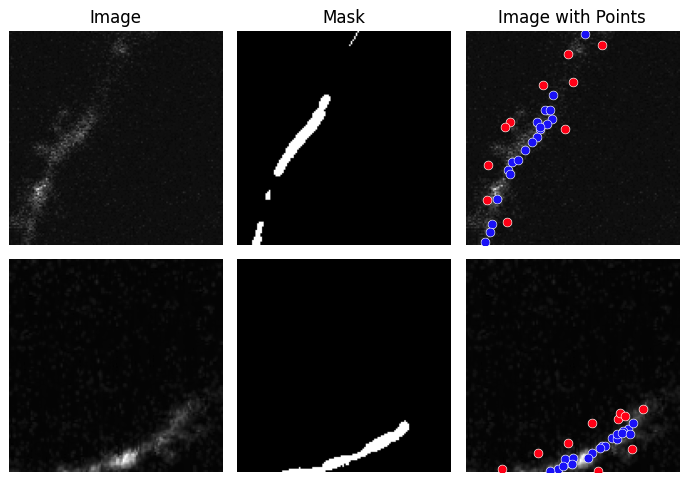
\includegraphics[width=0.9\textwidth]{figures/16_training_prompts.png}
\captionof{figure}{Prompt Points generated on the fly during training. The blue points show the positive (foreground) points and red points are the negative (background) points. Scale: $0.94\,\mu\text{m}/\text{px}$}
\label{fig:training_prompts}
\end{center}

\paragraph{Inference-Time Prompt Construction}

During inference in the Neuro-\gls{SAM} pipeline, the prompt strategy was fundamentally different: prompts were no longer randomly sampled, but rather derived directly from the manually traced dendritic path and its local context. The path, constructed interactively by the user, provided a spatial prior for where dendrites are expected to lie. For each 2D slice being segmented, the traced path was intersected with the corresponding image plane to extract candidate foreground (positive) points. These were projected into patch-local coordinates and, if needed, subsampled to ensure coverage while maintaining efficiency.

To complement these foreground prompts, background (negative) prompts were generated using a convex-hull-based envelope around the path. The algorithm constructed a narrow shell surrounding the positive region, defining an inner and outer boundary based on fixed radial distances. Negative points were then sampled from within this band, avoiding overlap with the dendrite core. This technique mimicked the negative prompt strategy used during training while adapting it to the path geometry produced by the user. If the convex hull could not be constructed (e.g., due to sparse waypoints), a fallback random sampling strategy was used instead. \autoref{fig:testing_prompts} shows the role of testing prompts. Positive prompts in the center of the dendrite (derived from the traced path) and a boundary region from where we sampled the negative prompts. It also shows how well the prompt points guide the model prediction on a patch from the benchmark dataset.

\begin{center}
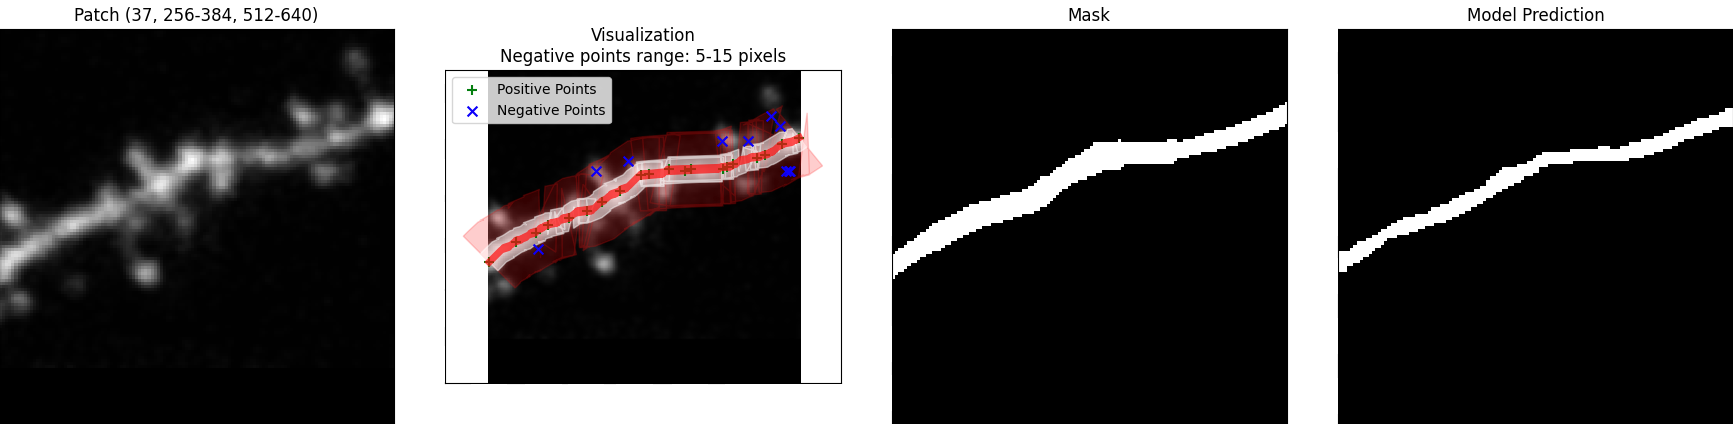
\includegraphics[width=1.0\textwidth]{figures/17_testing_prompts.png}
\captionof{figure}{Inference Prompt points along with model prediction. The first image shows the image patch, second shows the red region as foreground with a boundary region with negative points. The image third and fourth shows the ground truth and predicted mask. Scale: $0.94\,\mu\text{m}/\text{px}$}
\label{fig:testing_prompts}
\end{center}

Importantly, the prompts were not limited to a single slice. To improve robustness, particularly in anisotropic volumes, Neuro-\gls{SAM} allowed prompts to be collected from a small temporal window, typically $\pm 4$ slices around the current frame; thereby injecting limited 3D context into each segmentation operation without requiring full volumetric inference. This was particularly useful for guiding segmentation in frames with poor contrast or missing features.

In both training and inference, our prompt design emphasized \textit{locality}, \textit{structure-awareness}, and \textit{noise tolerance}, enabling \texttt{\gls{SAMv2}} to produce accurate segmentations that conform tightly to biological reality.

% \subsubsection{\textbf{Evaluation}}

% The fine-tuned \texttt{SAMv2} model for dendrite segmentation was evaluated on a dedicated validation split from our dataset, with benchmark stacks strictly excluded to preserve an unbiased test set for later pipeline-level assessment. Validation was performed every 500 training iterations and consisted of 20 randomly sampled batches, each processed without any form of augmentation to ensure metric consistency across epochs. The batch size for validation matched the training configuration to maintain comparable memory usage and computational load.

% Performance was quantified using a combination of pixel-level and object-level metrics. The primary segmentation accuracy measure was the Dice coefficient \cite{Shamir_2019}, chosen for its sensitivity to both precision and recall in binary mask prediction and its suitability for elongated structures such as dendrites. The Intersection-over-Union (IoU) \cite{Cheng_2021} was computed alongside Dice to provide a complementary perspective on mask overlap quality, particularly valuable for cases with small absolute foreground area. The total validation loss was also recorded, incorporating both the binary cross-entropy segmentation loss and the auxiliary score regression loss, enabling the tracking of not only spatial accuracy but also confidence calibration.

% For each validation batch, the predicted masks were binarized at a fixed threshold of 0.5 after sigmoid activation. The IoU was computed as:


% \[
% IoU = \frac{|P \cap G|}{|P \cup G|}
% \]

% where $P$ and $G$ denote the sets of predicted and ground truth foreground pixels, respectively. Meanwhile the Dice Score can be computed as:

% \[
% Dice = \frac{2 |P \cap G|}{|P| + |G|}
% \]

% These metrics were averaged at the end of 20 batches to yield mean validation scores for each evaluation step. In addition to numerical metrics, qualitative inspection was carried out by overlaying predicted masks on raw validation images, allowing rapid identification of common failure modes such as dendrite discontinuities or over-extension into background structures.

% The evaluation process played a critical role in model selection. Among the multiple variants trained during experimentation, the \texttt{SAMv2-small} model with 128$\times$128 input resolution was selected for integration into the Neuro-\gls{SAM} pipeline, as it consistently achieved a strong balance of high Dice/IoU scores, low validation loss, and rapid inference suitable for interactive annotation workflows.

\subsubsection{\textbf{Integration with Neuro-\gls{SAM} Pipeline}}

The fine-tuned \texttt{\gls{SAMv2}-small} model was fully embedded into the Neuro-\gls{SAM} interactive environment to enable seamless, localized dendrite segmentation directly within the existing dendrite tracing workflow. Once a user traces a dendritic path using the \textbf{Path Tracing Module}, the 3D coordinates of this path are used to define a spatially bounded \gls{ROI} within the anisotropic volume. This \gls{ROI} selection step is crucial, as it ensures that the segmentation model operates only on relevant sub-volumes, reducing inference time and minimizing false positives in unrelated regions.

Within this \gls{ROI}, the segmentation process follows the volumetric, overlapping patch-based inference strategy described earlier. The module divides each relevant frame into $128 \times 128$ pixel patches with a 50\% stride overlap, ensuring complete coverage of dendritic structures and robust handling of edge effects. Each patch is processed independently by the fine-tuned \texttt{\gls{SAMv2}} model using prompt points derived from the traced path, enabling localized predictions that align with the specific dendritic branch being segmented. The resulting patch-level masks are then merged via adaptive averaging, where pixel-level confidence thresholds are dynamically adjusted based on patch overlap counts to preserve structural continuity.

After merging, the raw binary masks undergo dendrite-specific post-processing. This includes hole filling to preserve the solid tubular morphology, morphological closing in both horizontal and vertical orientations to connect discontinuities, and removal of small isolated regions below a user-defined size threshold. Additionally, a path-proximity validation step discards any mask regions that deviate beyond a set spatial distance from the traced dendrite, effectively eliminating noise while retaining fine peripheral branches.

The segmented mask is immediately overlaid on the original 3D stack within the Napari-based Neuro-\gls{SAM} viewer, using a high-contrast color assigned to distinguish it from other dendrites and spines in the session. Users can interactively refine results by adjusting post-processing parameters, retracing path segments, or re-running segmentation with alternative patch sizes or prompt configurations. The final, validated masks can be exported as multi-frame TIFFs for downstream analysis or directly passed to subsequent modules in the pipeline.

By integrating the segmentation model in this tightly coupled manner, Neuro-\gls{SAM} ensures that dendrite segmentation is not a standalone step, but rather a fully interactive, path-aware process that naturally transitions into the spine detection module, where the segmented dendritic shafts form the structural basis for localized spine candidate generation.

\subsection{Spine Detection Module}

Detecting dendritic spines is an inherently challenging task due to their small size, morphological variability, and inconsistent contrast within noisy 3D microscopy volumes. To address this, the spine detection module in Neuro-\gls{SAM} employs a geometry-aware, intensity-guided pipeline that tightly couples with the previously traced dendritic paths. Rather than relying on conventional 3D blob detection or global segmentation strategies, this module performs localized dual-view analysis at discrete positions along the dendritic shaft. It extracts focused 2D views and orthogonal cross-sections collectively referred to as \textit{tube data} around each point along the traced path, enabling the system to identify spines with greater spatial and directional accuracy. Confirmed candidates are then refined through intensity consistency checks and spatial grouping, producing robust 3D coordinates for downstream segmentation. The resulting detections serve as direct input to the spine segmentation pipeline within Neuro-\gls{SAM}.

\subsubsection{\textbf{Tube Data Generation}}

To enable localized spine detection along the dendritic shaft, we construct a series of context-rich frames, termed \textit{tube data}, at equidistant points along the traced dendrite path. Each frame encodes local spatial information in both the axial (XY) and orthogonal cross-sectional directions referred to as \textit{tube data}. Given a discrete path \(\{\mathbf{p}_0, \mathbf{p}_1, \ldots, \mathbf{p}_{N-1}\}\) in 3D space, we compute tangent vectors via central differencing and derive a pair of orthonormal basis vectors \((\mathbf{up}_i, \mathbf{right}_i)\) at each location, defining a plane perpendicular to the local dendritic trajectory.

At every position \(\mathbf{p}_i\), three views are extracted:

\begin{itemize}
  \item A \textbf{zoomed patch} in the XY plane, centered at \(\mathbf{p}_i\), capturing local frontal features for 2D blob detection.
  \item A \textbf{tubular plane}, generated orthogonally to the dendrite axis using the basis vectors \(\mathbf{up}_i\) and \(\mathbf{right}_i\), for detecting off-axis structures.
  \item An optional \textbf{reference mask}, we got from the dendrite segmentations.
\end{itemize}

\begin{center}
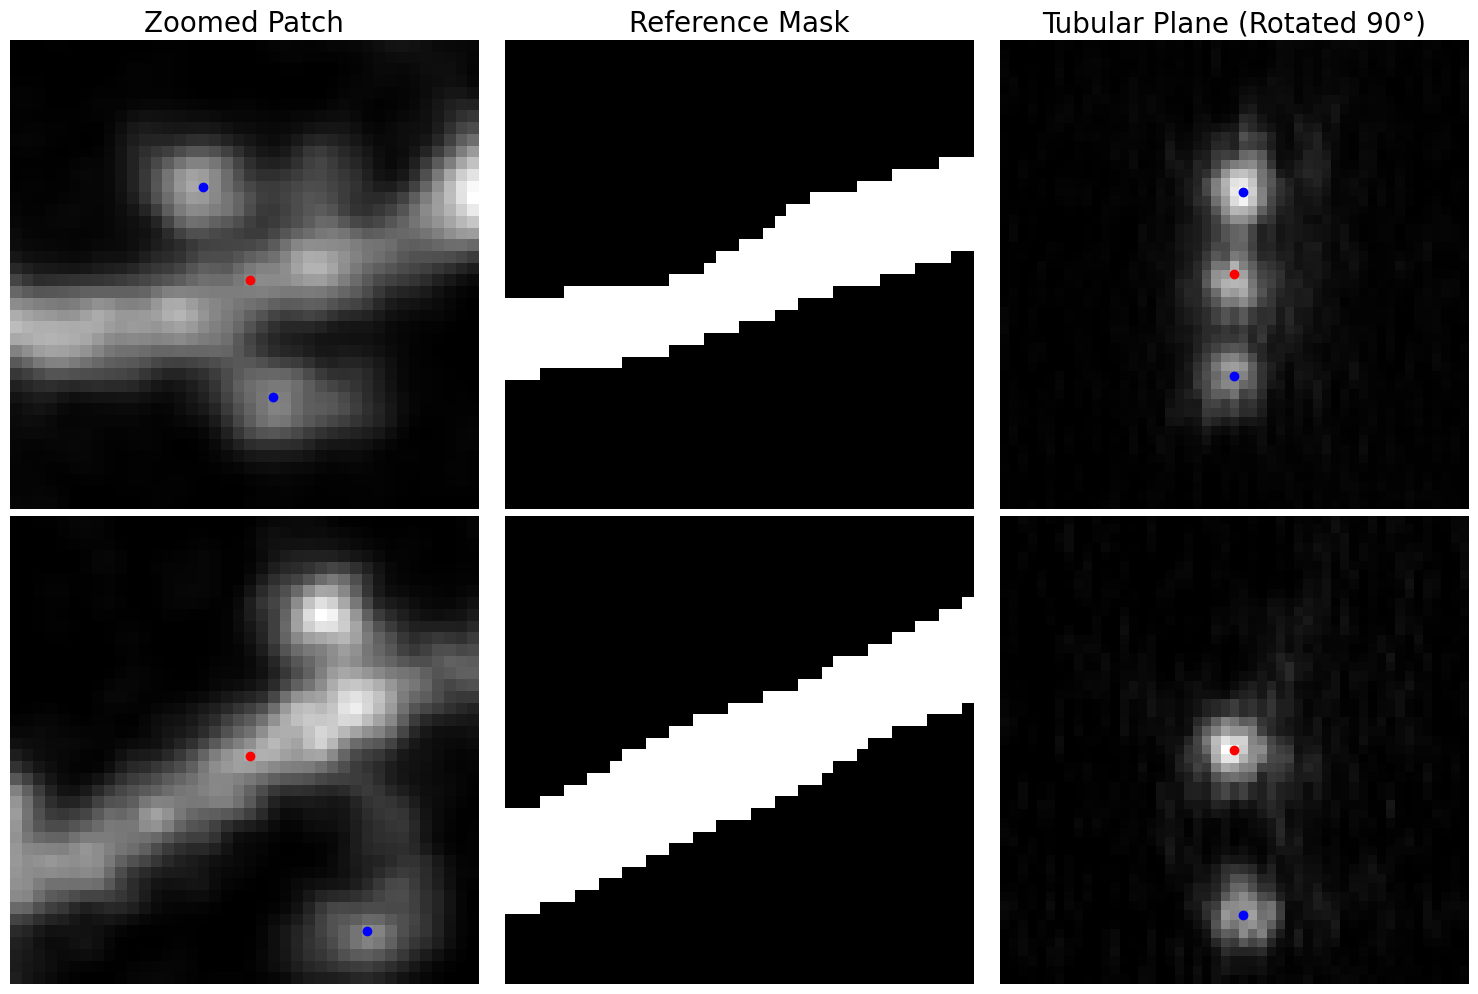
\includegraphics[width=0.8\textwidth]{figures/19_tube_data.png}
\captionof{figure}{The plot shows a 2D zoomed view of the dendrite, a reference mask and an in-tube view of the dendrite. The red point displays the center of the dendrite (obtained from path tracing), and the blue point displays the spines that are projecting outwards in the \gls{FOV}. Scale: $0.94\,\mu\text{m}/\text{px}$}
\label{fig:tube_data}
\end{center}

To compute the tubular plane, we define a 2D grid of size \((2w + 1) \times (2w + 1)\) centered on \(\mathbf{p}_i\), where \(w\) denotes the half-width in pixels. Each grid cell is mapped to a corresponding 3D coordinate in the original volume via:

\[
\mathbf{q}_{i,j,k} = \mathbf{p}_i + (j - w) \cdot \mathbf{up}_i + (k - w) \cdot \mathbf{right}_i,
\quad \text{where } j, k \in \{0, \ldots, 2w\}.
\]



These coordinates are rounded to the nearest voxel and sampled if within bounds. The resulting plane yields a cross-sectional slice orthogonal to the dendrite, faithfully aligned with its local direction of propagation.

This process is implemented using efficient, Numba-parallelized routines and supports reference blending for enhanced visualization. The full set of extracted frames constitutes the input to subsequent dual-view spine detection and geometric consistency filtering, detailed next.

\subsubsection{\textbf{Dual-View Spine Detection}}
Building on the localized \textit{tube data}, we now perform dual-view blob detection to identify dendritic spines. Global approaches often misinterpret fine structures near the shaft, so our method relies on spatially constrained, multi-view analysis for precise detection.

Each tube frame provides two complementary views to detect potential spine candidates. The first is the frontal 2D patch, a square XY slice centered on the dendritic path point. On this patch, we apply a \gls{LoG} \cite{Kong_2013} filter to highlight blob-like intensity structures. To avoid misidentifying the dendritic shaft itself, we subtract a reference mask before detection, effectively suppressing the central dendritic region. In parallel, we apply a similar \gls{LoG}-based detection on the \textit{tubular view}. This orthogonal detection step captures spines that may not be prominent in the frontal XY plane due to orientation or noise. The outputs of this step are candidate blob coordinates identified in the tubular view, relative to the orientation of the dendrite at each point.

To consolidate detections from both views, we perform pairwise matching between 2D frontal blobs and tubular blobs based on geometric consistency. For each frontal candidate, we compute its direction vector relative to the center of the patch and compare it with the local dendrite orientation at that frame. Similarly, each tubular blob is represented by a vector from the center of the tubular plane. These vectors are converted to angles, and angular consistency is computed via dot product and cross product formulations. Only pairs with angular differences below a defined threshold (typically \(20^\circ\text{–}25^\circ\) are considered.

The Euclidean distance of each blob from the patch center is compared across both views. The matching score for a pair is computed as a weighted combination of angular difference and distance mismatch, controlled by an angle-weighting hyperparameter (e.g., 0.7). The best-matching tubular blob for each 2D frontal blob is selected, and only those with scores below a strict threshold are retained as confirmed candidates. This cross-view verification ensures that final spine detections are not only morphologically plausible, but also directionally consistent with the underlying dendritic shaft.

Following the initial detection, spine candidates are grouped based on spatial proximity in the lateral plane to merge redundant detections across adjacent frames. Within each group, the most structurally distinct instance, typically the brightest or most contrasted is selected. This spine is then re-evaluated across neighboring slices to assess its visibility using localized intensity analysis. Only those candidates consistently distinguishable from the background are retained. The final set of tracked spines is both spatially unique and temporally validated, ensuring reliable input for the downstream segmentation module.

While the automated detection pipeline captures the majority of spine candidates, Neuro-\gls{SAM} also allows users to manually annotate spines via interactive point placement within the 3D interface. These manual inputs are treated identically to algorithmic detections, integrated into the tracking and refinement workflow without distinction. This ensures flexibility in handling edge cases or atypical morphologies that escape automated detection. With a finalized set of spatially verified spine coordinates, we next shift focus to the segmentation of these structures, where localized prompts are leveraged to extract fine-grained spine masks.

\subsubsection{\textbf{Spine Detection Algoritm (Pseudocode)}}

The entire spine detection workflow is summarized in Algorithm \ref{alg:spine_detection}, which outlines the key steps from dual-view blob extraction and angle-based matching to manual integration and final tracking with intensity-aware validation. This procedure ensures spatially consistent and morphologically relevant spine candidates, ready for downstream segmentation.

\begin{algorithm}[htb]
\footnotesize
\begin{algorithmic}[1]
    \State \textbf{Input:} 3D image volume $\mathcal{I}$, traced dendrite path $\mathcal{P}$, segmentation mask $\mathcal{M}$, optional manual points $\mathcal{U}$
    \State \textbf{Output:} 3D spine coordinates $\mathcal{S}$

    \State 
    \State \textbf{Step 1: Tube Data Construction}
    \For{each path point $\mathbf{p}_i \in \mathcal{P}$}
        \State Compute tangent vector using central difference
        \State Generate local orthonormal basis $(\mathbf{up}_i, \mathbf{right}_i)$
        \State Sample:
        \State \hspace{1em} (a) Frontal XY patch centered at $\mathbf{p}_i$
        \State \hspace{1em} (b) Orthogonal tubular plane via coordinate projection
        \State \hspace{1em} (c) Reference patch from $\mathcal{M}$ (optional)
        \State Store all three views in frame data $\mathcal{T}[i]$
    \EndFor

    \State 
    \State \textbf{Step 2: Spine Blob Detection}
    \For{each frame $t \in \mathcal{T}$}
        \State Apply LoG blob detection on frontal patch
        \State Apply LoG blob detection on tubular plane 
        \State Extract blob coordinates in both views
    \EndFor

    \State 
    \State \textbf{Step 3: Angle-Based Matching Across Views}
    \For{each frontal blob in frame $t$}
        \For{each tubular blob in the same frame}
            \State Compute relative angle with dendrite tangent
            \State Compute radial distance from view center
            \State If both angle and distance criteria are satisfied:
            \State \hspace{1em} Add to list of matched spine candidates
        \EndFor
    \EndFor

    \State 
    \State \textbf{Step 4: Manual Point Integration}
    \If{manual spine points $\mathcal{U}$ are provided}
        \State Merge $\mathcal{U}$ with matched spine candidates
    \EndIf

    \State 
    \State \textbf{Step 5: Spine Tracking}
    \State Group nearby spines across frames to avoid duplicates
    \For{each spine group}
        \State Select representative spine based on intensity
        \State Track visibility across neighboring Z-slices
        \If{visible in any frame}
            \State Add frame-local positions to final spine list $\mathcal{S}$
        \EndIf
    \EndFor

    \State 
    \State \Return Final spine coordinates $\mathcal{S}$
\end{algorithmic}
\caption{Spine Detection using Dual-View Matching and Intensity-Aware Tracking}
\label{alg:spine_detection}
\end{algorithm}

\subsection{Spine Segmentation Module}
While dendrite segmentation provides the structural backbone for Neuro-\gls{SAM}, accurate segmentation of individual dendritic spines requires a separate, specialized treatment. These micron-scale protrusions exhibit high shape variability, low contrast, and often cluster near dense dendritic regions posing a substantial challenge for segmentation algorithms. To address this, we fine-tuned a dedicated instance of \texttt{SAMv2} specifically for spine segmentation using candidate-aware prompts and overlapping patch-based inference. Unlike dendrites, spine masks tend to be sparse, disconnected, and morphologically heterogeneous, demanding both precise center localization and shape-aware post-processing. Our model operates on localized \gls{ROI}s defined by the previously detected spine candidates, optionally enriched with manual point corrections, and leverages the model's internal morphological priors to produce clean, circular spine masks suitable for downstream analysis and quantification.

% \subsubsection{\textbf{Dataloader}}
% For training the spine segmentation model, we developed a custom streaming dataloader, \texttt{SpineGeneratorStream}. This dataloader dynamically samples 2D patches from randomly selected 3D volumes and resizes each patch to 128$\times$128 pixels while preserving a fixed spatial resolution of 94~nm/pixel using voxel metadata. Only samples with at least 100 pixels of annotated dendritic or spine content were retained, ensuring that the model was consistently exposed to informative training regions.

% Each training sample comprises three aligned channels: the raw image patch, a binary dendrite mask, and a corresponding binary spine mask. These masks are used not only for supervision but also for generating training prompts on-the-fly. Data augmentation is performed in real-time using a composite of geometric (rotations, flips), photometric (brightness, contrast), and noise-based transformations via \texttt{Albumentations}. This dynamic pipeline enables highly diverse training while avoiding redundant disk-based patch storage.

% To facilitate point-based segmentation learning, the dataloader invokes a lightweight \texttt{PromptGeneration} module that identifies candidate spine centers. It uses distance-transform and watershed segmentation to identify spine center and separate connected spines. These detected centers are converted into positive prompts, while optional background points are sampled from non-spine regions to guide the model in suppressing false positives. This prompt generation is both patch-local and density-aware, enabling flexible supervision even in crowded spine environments.

\subsubsection{\textbf{Fine-Tuning Setup}}

The spine segmentation model was fine-tuned on the \texttt{\gls{SAMv2}} architecture, targeting localized instance segmentation of dendritic spines using patch-wise point prompts. Unlike the dendrite segmentation pipeline, which required broader path-aware regions, spine segmentation focused exclusively on sparse object centers, enabling us to train using a single-point prompt strategy without additional bounding boxes or masks. Data loading, pre-processing, data augmentation, and prompt feeding was carried out by a \texttt{SpineGeneratorStream} that loaded 2D slices from the dataset. 

Two \texttt{\gls{SAMv2}} model variants were evaluated during experimentation: \texttt{\gls{SAMv2}-small} and \texttt{\gls{SAMv2}-large}, each tested with input image resolutions of 128$\times$128, 512$\times$512, and 1024$\times$1024. This allowed us to study the effect of receptive field size and backbone capacity on small object segmentation in cluttered dendritic contexts. Although the large model offered marginal gains at higher resolutions, it incurred a significant memory overhead. Ultimately, the \texttt{\gls{SAMv2}-small} model at 128$\times$128 input resolution was selected, offering optimal trade-offs between segmentation quality and computational efficiency in high-throughput settings. Rest, all the parameter such as optimizer, learning rate, weight decya were kept the same as dendrite segmentation module. 

% Fine-tuning was conducted end-to-end using the full \gls{SAMv2} pipeline. The image encoder, prompt encoder, and mask decoder were all kept trainable. To support mixed-precision training, we employed PyTorch's \texttt{torch.amp} for automatic casting and gradient scaling. The optimizer used was \texttt{AdamW} \cite{Loshchilov_2019} with a learning rate of $1 \times 10^{-5}$ and weight decay of $4 \times 10^{-5}$, consistent with the dendrite training regime to maintain compatibility across modules.

During each training iteration, the model received a batch of single image patch, its binary spine mask, and a corresponding set of spine center prompts were generated. Each prompt was encoded as a positive point input to the \texttt{\gls{SAMv2}} prompt encoder and combined with the high-resolution image embeddings for mask prediction. Unlike the dendrite model, which leveraged both positive and negative prompts, the spine model was trained using only foreground (positive) points due to the isolated nature of spine centers and their weak boundary contrast.

The loss function consisted of two components: (i) a binary cross-entropy loss between predicted and ground truth spine masks, and (ii) a score regression loss that penalized the absolute deviation between the predicted confidence score and the ground truth \gls{IoU}, scaled by 0.05. These were aggregated into a composite loss, ensuring that both segmentation shape and model confidence were jointly optimized.
Fine-tuning was performed for 100,000 iterations with a batch size of 32. Checkpoints were saved periodically, and all performance metrics were logged using Weights \& Biases for real-time monitoring.

\subsubsection{\textbf{Prompt Strategy for Spines}}
We employed two tailored prompt strategies, one during training and another during inference, both based on single-point supervision, which proved optimal for localizing small, variable spines.

\textbf{Training-Time Prompt Generation }
For training, positive point prompts were generated by computing the distance transform of each spine mask and selecting the central peak as the foreground point. Watershed labels were used to separate two joined spines. No negative prompts were used, as they introduced ambiguity in crowded or poorly segmented regions. \autoref{fig:spine_training_prompts} shows an example of how the prompt points look like for the dendritic spines during training. This point-based supervision strategy was implemented directly within the \texttt{SpineGeneratorStream}, ensuring alignment with the model’s segmentation objectives. Patches varied in spine density, allowing the model to generalize across both sparse and clustered regions.

\begin{center}
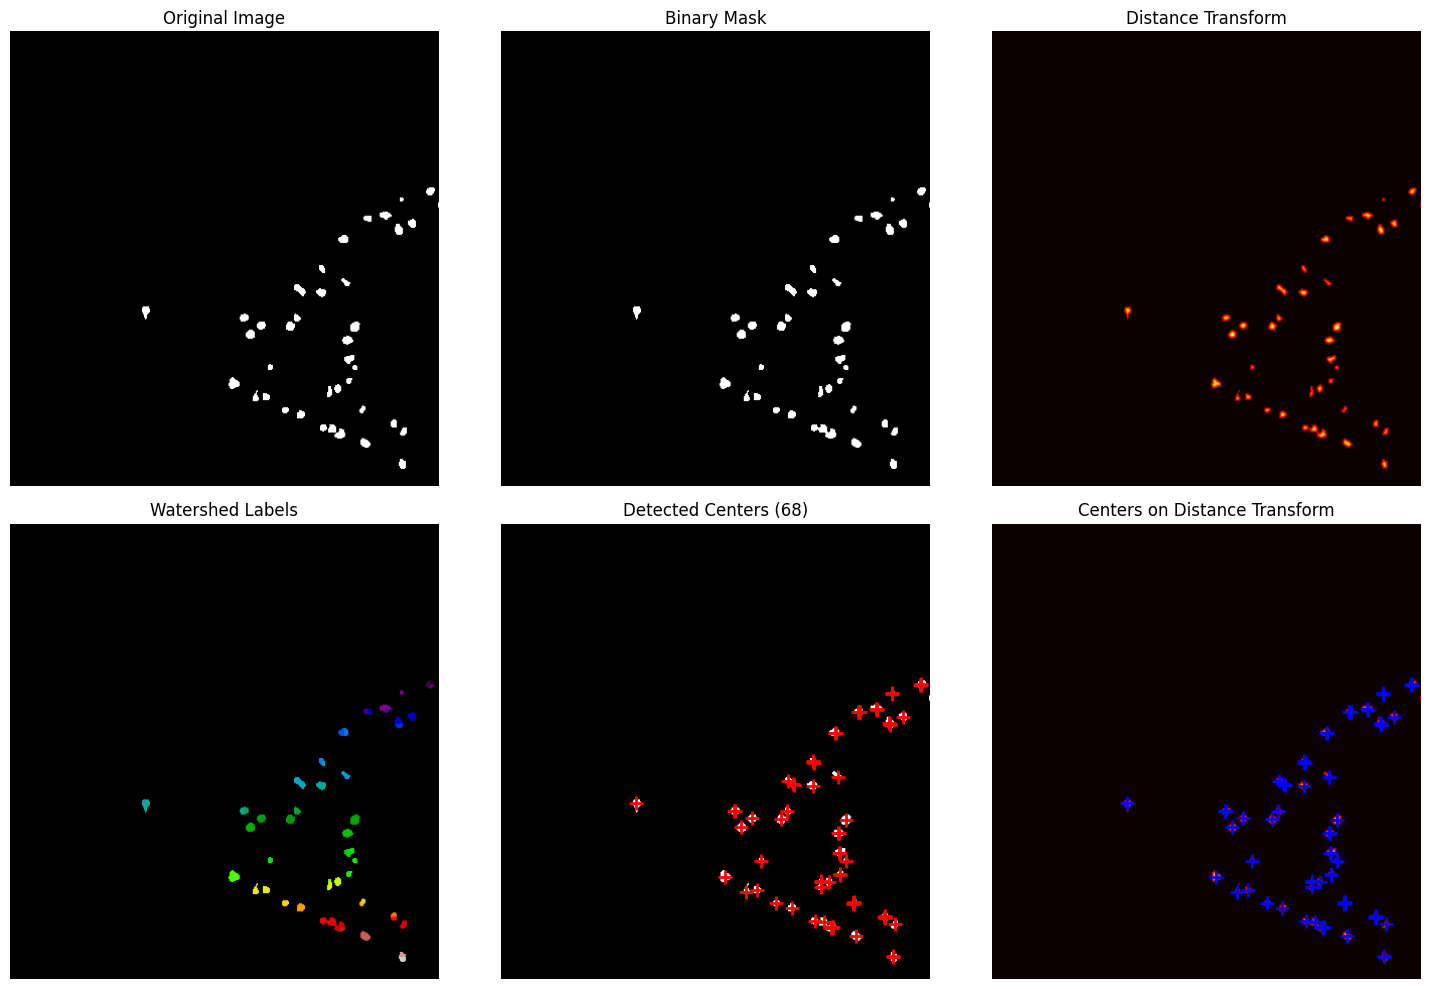
\includegraphics[width=0.95\textwidth]{figures/18_spine_prompt_training.png}
\captionof{figure}{Figure shows the process of finding positive prompts points from spines masks. Spine Centers are found using distance transform, connected spines are separated using watershed labels, combined together forms the positive prompts for the model. Scale: $0.94\,\mu\text{m}/\text{px}$}
\label{fig:spine_training_prompts}
\end{center}

\paragraph{Inference-Time Prompt Strategy}

During inference, spine locations are either detected automatically from \textit{Spine Detection Module} or added manually were used directly as positive prompts. \autoref{fig:tube_data} shows an example of detected spines across two patches. Each 3D coordinate was projected into 2D frames and fed into the \gls{SAMv2} prompt encoder without modification, maintaining consistency with the training distribution. For manual annotations, the \texttt{SpineTracker} extended prompts across adjacent frames to capture anisotropic spines. This unified, point-based strategy enabled the model to generate focused spine masks with high spatial precision.

\subsubsection{\textbf{Evaluation}}
Similar to the dendrite segmentation, the spine segmentation model was evaluated on a fixed validation split from the dataset, strictly excluding benchmark stacks. Every 500 iterations during training, validation was performed over 20 batches, each comprising 128$\times$128 patches without augmentation to ensure consistency. Predictions were thresholded at 0.5 after sigmoid activation and performance was quantified using the Dice coefficient and \gls{IoU} metrics.

Among all trained variants, the \texttt{\gls{SAMv2}-small} model at 128 resolution consistently achieved the best trade-off between speed and performance. Larger models and higher resolutions showed marginal improvements in Dice and \gls{IoU} but introduced considerable memory and runtime overhead without yielding biologically relevant benefits. The final selected model achieved stable performance with fast inference, making it suitable for integration into interactive annotation workflows.

\subsubsection{\textbf{Integration into Neuro-\gls{SAM} Pipeline}}
The spine segmentation model is tightly integrated into the Neuro-\gls{SAM} workflow. After spine candidates are confirmed, 128$\times$128 patches are extracted around each spine and processed using the fine-tuned \texttt{\gls{SAMv2}-small} model. Foreground prompts are derived from spine centers, with optional dendrite-based suppression.

The model handles segmentation and post-processing internally. Overlapping predictions are merged adaptively and visualized directly in the Napari viewer, with contrasting colors for clarity. Each segmented spine is rendered with a high-contrast color and users can interactively inspect, correct, or export the final results. This tightly coupled design ensures that spine segmentation is not a standalone operation, but rather a seamless continuation of the detection workflow anchored to biological structure and visual feedback.

The Neuro-\gls{SAM} pipeline brings together four tightly integrated modules: path tracing, dendrite segmentation, spine detection, and spine segmentation into a coherent and interactive system for annotating dendritic structures in 3D microscopy volumes. Each module operates independently but communicates contextual signals to maintain spatial and semantic consistency. By combining foundation models like \texttt{\gls{SAMv2}} with patch-wise inference, custom prompt logic, and real-time interaction, the system achieves fine-grained, high-fidelity predictions with minimal manual input.

With the technical foundations in place and the modular design firmly established, the discussion now shifts toward empirical evaluation. The next section focuses on how these methods perform in practice, analyzing their quantitative accuracy, robustness across datasets, and overall annotation efficiency.

